\section{Construção {\it online} da {\it trie}}

\begin{frame}[fragile]{Algoritmo {\it online} para construção de uma {\it trie}}

    \begin{itemize}
        \item A construção pode ser melhorada por meio de um algoritmo \textit{online}
        \pause

        \item A ideia principal é, ao invés de construir toda a \textit{trie} de $s$ de uma só 
            vez, construí-la a partir da \textit{trie} de $s[1..(N-1)]$ 
        \pause

        \item Seja $T_j$ a \textit{trie} do prefixo $s[1..j]$ de $s$ 
        \pause

        \item A principal observação a ser feita é que $T_j$ pode ser construída a partir da 
            inserção do caractere $s[j]$ em $T_{j - 1}$, nas arestas dos novos nós a serem 
            adicionados aos nós essenciais de $T_{j - 1}$, quando for o caso
        \pause

        \item Isto acontecerá quando o nó essencial não tem um filho ligado a ele por meio de 
            uma aresta cujo rótulo é $s[j]$
        \pause

        \item O ponto principal, portanto, se torna determinar a sequência dos nós essenciais 
            $v_k, v_{k-1}, \ldots, v_2, v_1, v_0$, onde $v_i$ corresponde ao prefixo 
            $s[1..i]$ de $T_k$
        \pause

        \item Esta tarefa pode ser feita por meio do uso de \textit{links} de sufixos
    \end{itemize}

\end{frame}

\begin{frame}[fragile]{{\it Links} de sufixos}

    \begin{itemize}
        \item Seja $u$ um nó de $T_k$
        \pause

        \item Defina o \textit{link} de sufixo $suf(u) = v$, onde $v$ é um nó cujo caminho 
            $p(v)$ da raiz até $v$ é igual 
            ao caminho de $[2..p(u)]$, isto é, o caminho $p(u)$ sem o seu primeiro caractere
        \pause

        \item Por definição, se a raiz de $T_k$ corresponde ao vértice $v_0$, então 
            $suf(v_0) = v_0$
        \pause

        \item Contudo, interpretar $suf(v_0)$ como \code{cpp}{nullptr} pode ser mais 
            interessante na implementação do algoritmo
        \pause

        \item Esta definição leva a igualdade
        \[
            (v_k, v_{k-1}, \ldots, v_0) = (v_k, suf(v_k), suf^2(v_k), \ldots, suf^{k - 1}(v_k))
        \]

    \end{itemize}

\end{frame}

\begin{frame}[fragile]{Visualização dos {\it links} de sufixos da {\it trie} da palavra {\tt `BANANA'}}

    \begin{figure}
        \centering

        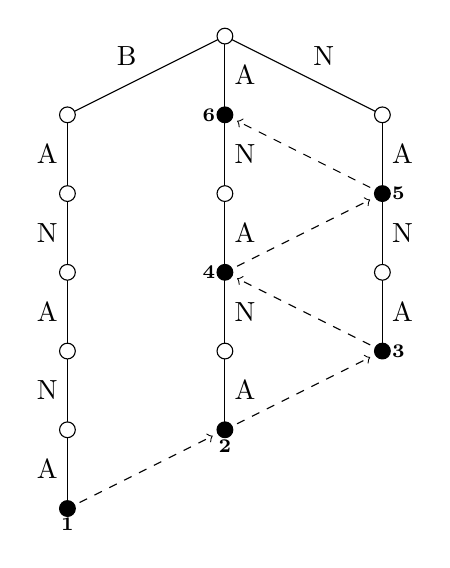
\begin{tikzpicture}
            \coordinate (A) at (4, 7);
            \coordinate (B1) at (2, 6);
            \coordinate (B2) at (4, 6);
            \coordinate (B3) at (6, 6);
            \coordinate (C1) at (2, 5);
            \coordinate (C2) at (4, 5);
            \coordinate (C3) at (6, 5);
            \coordinate (D1) at (2, 4);
            \coordinate (D2) at (4, 4);
            \coordinate (D3) at (6, 4);
            \coordinate (E1) at (2, 3);
            \coordinate (E2) at (4, 3);
            \coordinate (E3) at (6, 3);
            \coordinate (F1) at (2, 2);
            \coordinate (F2) at (4, 2);
            \coordinate (G1) at (2, 1);

            \draw (A) -- node[anchor=south east] { B } (B1);
            \draw (A) -- node[anchor=west] { A } (B2);
            \draw (A) -- node[anchor=south west] { N } (B3);
            \draw (B1) -- node[anchor=east] { A } (C1);
            \draw (B2) -- node[anchor=west] { N } (C2);
            \draw (B3) -- node[anchor=west] { A } (C3);
            \draw (C1) -- node[anchor=east] { N } (D1);
            \draw (C2) -- node[anchor=west] { A } (D2);
            \draw (C3) -- node[anchor=west] { N } (D3);
            \draw (D1) -- node[anchor=east] { A } (E1);
            \draw (D2) -- node[anchor=west] { N } (E2);
            \draw (D3) -- node[anchor=west] { A } (E3);
            \draw (E1) -- node[anchor=east] { N } (F1);
            \draw (E2) -- node[anchor=west] { A } (F2);
            \draw (F1) -- node[anchor=east] { A } (G1);

            \draw[fill=white] (A) circle [radius=.1];

            \node[circle] (N1) at (G1) { };
            \node[circle] (N2) at (F2) { };
            \node[circle] (N3) at (E3) { };
            \node[circle] (N4) at (D2) { };
            \node[circle] (N5) at (C3) { };
            \node[circle] (N6) at (B2) { };

            \draw[dashed,->] (N1) -- (N2);
            \draw[dashed,->] (N2) -- (N3);
            \draw[dashed,->] (N3) -- (N4);
            \draw[dashed,->] (N4) -- (N5);
            \draw[dashed,->] (N5) -- (N6);

            \draw[fill=white] (B1) circle [radius=.1];
            \draw[fill=black] (B2) circle [radius=.1] node[anchor=east] { \scriptsize \bf 6 };
            \draw[fill=white] (B3) circle [radius=.1];
            \draw[fill=white] (C1) circle [radius=.1];
            \draw[fill=white] (C2) circle [radius=.1];
            \draw[fill=black] (C3) circle [radius=.1] node[anchor=west] { \scriptsize \bf 5 };
            \draw[fill=white] (D1) circle [radius=.1];
            \draw[fill=black] (D2) circle [radius=.1] node[anchor=east] { \scriptsize \bf 4 };
            \draw[fill=white] (D3) circle [radius=.1];
            \draw[fill=white] (E1) circle [radius=.1];
            \draw[fill=white] (E2) circle [radius=.1];
            \draw[fill=black] (E3) circle [radius=.1] node[anchor=west] { \scriptsize \bf 3 };
            \draw[fill=white] (F1) circle [radius=.1];
            \draw[fill=black] (F2) circle [radius=.1] node[anchor=north] { \scriptsize \bf 2 };
            \draw[fill=black] (G1) circle [radius=.1] node[anchor=north] { \scriptsize \bf 1 };

        \end{tikzpicture}
    \end{figure}

\end{frame}

\begin{frame}[fragile]{Construção {\it online} da {\it trie}}

    A construção \textit{online} de $T_k$ a partir de $T_{k-1}$ pode ser feita por meio dos 
    seguintes passos:
        \pause

    \begin{enumerate}
        \item identifique os nós essenciais $v_{k-1}, v_{k-2}, \ldots, v_1, v_0$ de $T_{k-1}$,
        em ordem decrescente em relação ao tamanho do sufixo relacionado
        \pause

        \item escolha os nós $v_i$ consecutivos até que se atinja um nó $v_t$ tal que exista um 
            filho de $v_t$ unido por uma aresta cujo rótulo é $s[k]$
        \pause

        \item para cada um dos nós escolhidos, crie novos nós filhos ligados por arestas 
            cujos rótulos sejam $s[k]$
        \pause

        \item atualize os \textit{links} de sufixos para os novos nós recém-criados
    \end{enumerate}

\end{frame}

\input{trie_online_view}

\begin{frame}[fragile]{Implementação da construção {\it online} da {\it trie}}
    \inputsnippet{cpp}{9}{26}{codes/trie_online.cpp}
\end{frame}

\begin{frame}[fragile]{Implementação da construção {\it online} da {\it trie}}
    \inputsnippet{cpp}{27}{46}{codes/trie_online.cpp}
\end{frame}

\begin{frame}[fragile]{Implementação da construção {\it online} da {\it trie}}
    \inputsnippet{cpp}{48}{53}{codes/trie_online.cpp}
\end{frame}

\begin{frame}[fragile]{Considerações sobre a construção {\it online} da {\it trie}}

    \begin{itemize}
        \item Observe que, na implementação proposta, os valores $v_k$ são usandos implicitamente
        \pause

        \item Para uma string $s$ de tamanho $n$, a construção \textit{online} da \textit{trie}
            tem complexidade $O(|T_n|)$
        \pause

        \item Embora ainda não seja a complexidade desejada ($O(n)$), esta estratégia será 
            pode ser utilizada, com alguns ajustes, para atingir tal complexidade
        \pause

        \item Para reduzir o tamanho em memória da \textit{trie} uma estratégia possível é 
            compactar as cadeias, onde uma cadeia é o maior caminho possível composto por nós 
            não-essenciais com grau de saída um 
        \pause

        \item Esta compactação resulta em uma nova estrutura, denominada \textit{suffix tree}
    \end{itemize}

\end{frame}
